
\documentclass[tikz,border=2mm]{standalone}
\usepackage[utf8]{inputenc}
\usepackage[T1]{fontenc}
\usepackage{amsmath}
\usepackage{amssymb}
\usetikzlibrary{arrows.meta,positioning,calc,shapes.geometric}
\usepackage{xcolor}

\definecolor{inkNavy}{HTML}{1B2733}
\definecolor{slate}{HTML}{3B4B5C}
\definecolor{paper}{HTML}{FBFAF7}
\definecolor{amber}{HTML}{C97A2B}
\definecolor{teal}{HTML}{2E7D74}
\definecolor{softred}{HTML}{A6402F}
\definecolor{lightgrey}{HTML}{E7E4DD}
\definecolor{midgrey}{HTML}{8B8A85}

\begin{document}
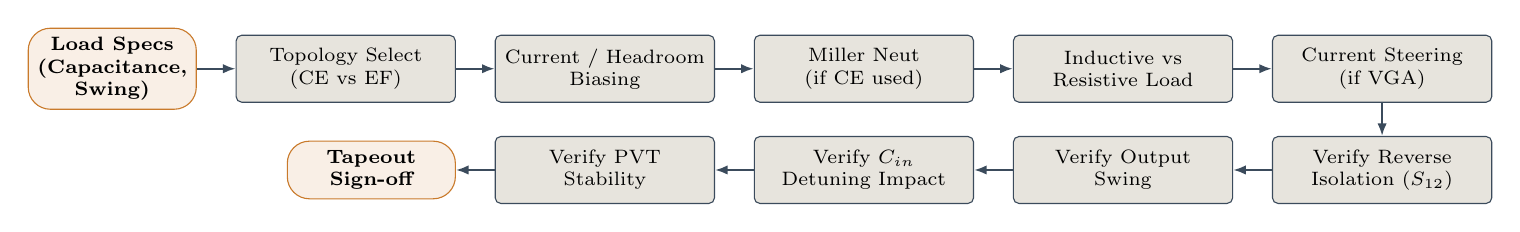
\begin{tikzpicture}[
  node distance=6pt and 14pt,
  box/.style={draw=slate, fill=lightgrey, rounded corners=2pt, text width=2.55cm, align=center, minimum height=0.85cm, font=\scriptsize},
  term/.style={draw=amber, fill=amber!12, rounded corners=8pt, text width=1.9cm, align=center, minimum height=0.7cm, font=\scriptsize\bfseries},
  arr/.style={-{Latex[length=1.6mm]}, slate, thick}
]
\node[term] (spec) {Load Specs\\(Capacitance, Swing)};
\node[box, right=of spec] (top) {Topology Select\\(CE vs EF)};
\node[box, right=of top] (bias) {Current / Headroom\\Biasing};
\node[box, right=of bias] (neut) {Miller Neut\\(if CE used)};
\node[box, right=of neut] (load) {Inductive vs\\Resistive Load};
\node[box, right=of load] (vga) {Current Steering\\(if VGA)};

\node[box, below=12pt of vga] (iso) {Verify Reverse\\Isolation ($S_{12}$)};
\node[box, left=of iso] (swing) {Verify Output\\Swing};
\node[box, left=of swing] (cin) {Verify $C_{in}$\\Detuning Impact};
\node[box, left=of cin] (pvt) {Verify PVT\\Stability};
\node[term, left=of pvt] (fin) {Tapeout\\Sign-off};

\draw[arr] (spec)--(top); \draw[arr] (top)--(bias); \draw[arr] (bias)--(neut);
\draw[arr] (neut)--(load); \draw[arr] (load)--(vga); \draw[arr] (vga)--(iso);
\draw[arr] (iso)--(swing); \draw[arr] (swing)--(cin); \draw[arr] (cin)--(pvt);
\draw[arr] (pvt)--(fin);
\end{tikzpicture}
\end{document}